    \section{Scalable Processing of Moving Flock Patterns}

    \begin{frame}{Large trajectory databases}
        \begin{minipage}{0.59\textwidth}
            \begin{itemize}
                \item A spatial trajectory is a trace in time generated by a moving entity in a geographical space.
                \item i.e. $p_1 \rightarrow p_2 \rightarrow \cdots \rightarrow p_n$
                \item A trajectory is stored as a time-ordered sequence of points, $p_i = (x, y, t)$ (spatial coordinate + time stamp).
            \end{itemize}
        \end{minipage}\hfill % maximize the horizontal separation
        \begin{minipage}{0.4\textwidth}
            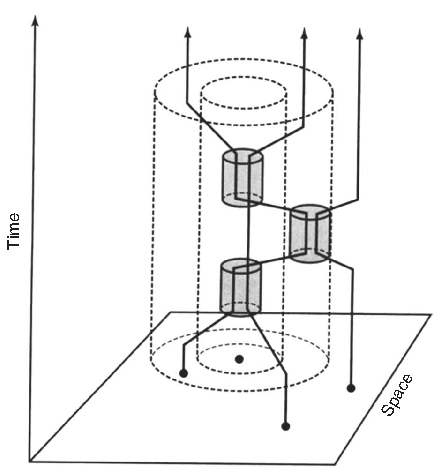
\includegraphics[width=\textwidth]{figures/trajectory}
            \begin{flushright}
                {\tiny (Shoval, 2017)}
            \end{flushright}
        \end{minipage}
    \end{frame}

    \begin{frame}{Movement patterns}
        \centering
        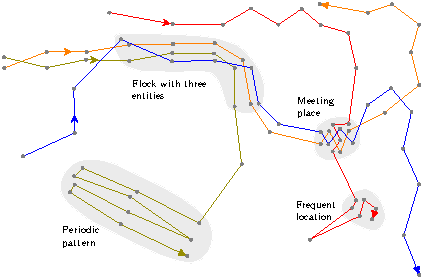
\includegraphics[width=0.75\textwidth]{figures/Patterns/patterns}
        \begin{flushright}
            {\tiny (Gudmundsson, et al. 2008)}
        \end{flushright}


        \begin{itemize} \item i.e. convoys, moving clusters, swarms, gatherings, \textbf{flocks}, ... \end{itemize} \vspace{0.5cm}
    \end{frame}

    \begin{frame}{Flocks}
        \centering
        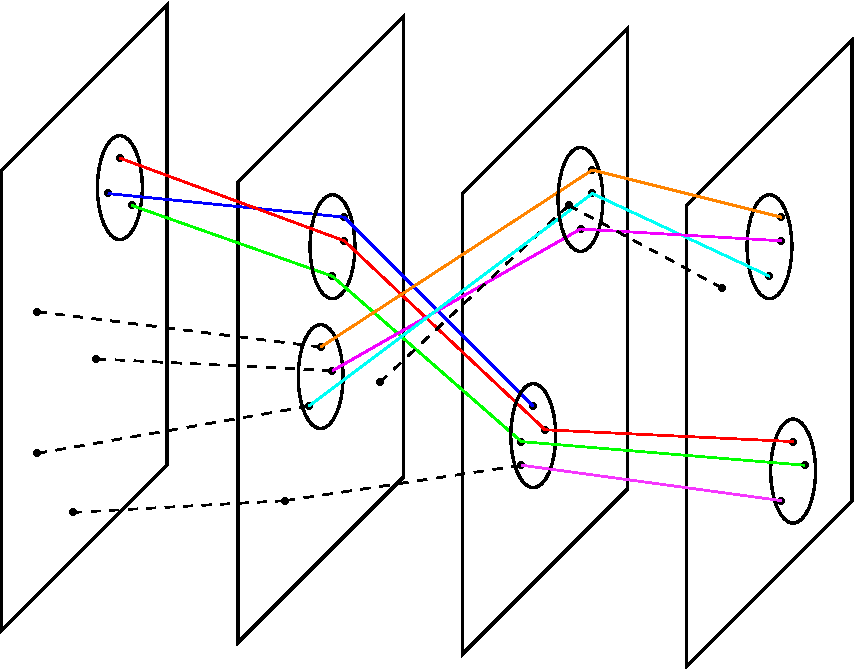
\includegraphics[width=0.55\textwidth]{figures/flock}

        \begin{itemize}
            \item $\varepsilon$: Diameter of the circle which contains all the objects.
            \item $\mu$: Minimum number of objects.
            \item $\delta$: Minimum time interval the objects travel `together'.
        \end{itemize}
    \end{frame}

    \begin{frame}{\textbf{B}asic \textbf{F}lock \textbf{E}valuation algorithm}
        \begin{itemize}
            \item Vieira, et al. 2009.
            \item The first polynomial-time solution for determining disk locations.
            \item Under fixed time duration it has polynomial time complexity $O(\delta|\tau|^{(2\delta) + 1})$
        \end{itemize}
        \vspace{0.25cm}

        \centering
        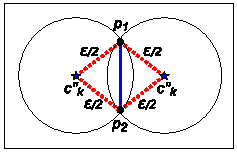
\includegraphics[width=0.5\textwidth]{figures/theorem}

    \end{frame}

    \begin{frame}{\textbf{B}asic \textbf{F}lock \textbf{E}valuation algorithm}
        \begin{itemize}
            \item Two main parts:
            \begin{itemize}
                \item In the spatial domain it finds maximal disks at each time instant.
                \item In the temporal domain it joins consecutive times to match set of maximal disks.
            \end{itemize}
        \end{itemize}
    \end{frame}

    \begin{frame}{On the spatial domain}
        \begin{itemize} \item BFE overview... \end{itemize} \vspace{0.5cm}

        \centering
        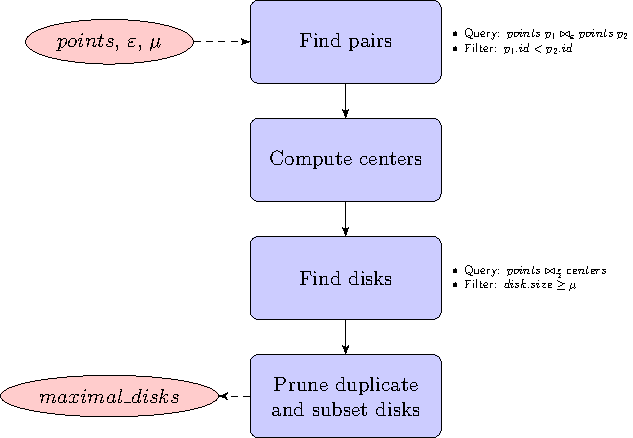
\includegraphics[width=0.7\textwidth]{../thesis/chapterPFlocks/figures/MF_flowchart}
    \end{frame}

    \begin{frame}{On the spatial domain}
        \begin{itemize} \item BFE overview... \end{itemize} \vspace{0.5cm}

        \centering
        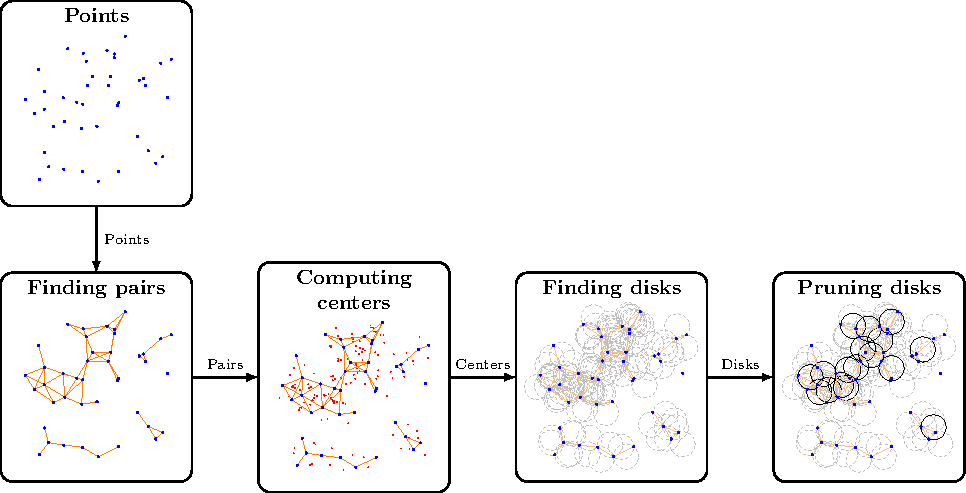
\includegraphics[width=\textwidth]{../thesis/chapterPFlocks/figures/MF_stages2/flow}
    \end{frame}

    \begin{frame}{On the temporal domain}
        \begin{itemize} \item BFE overview... \end{itemize} \vspace{0.5cm}

        \centering
        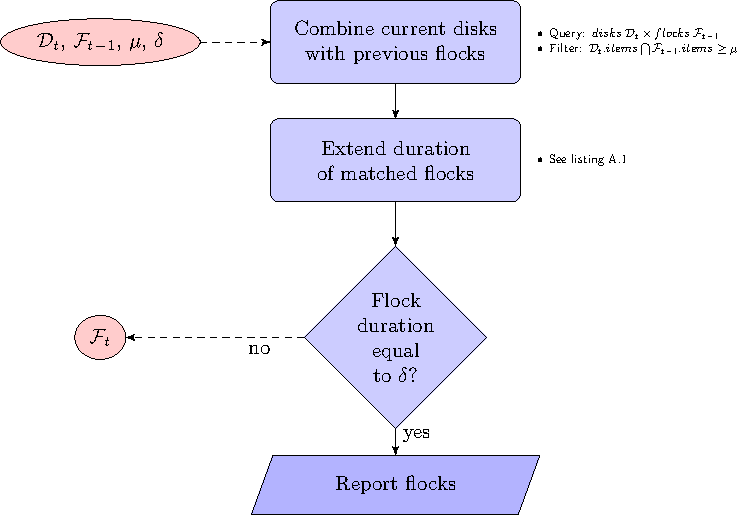
\includegraphics[width=0.7\textwidth]{../thesis/chapterPFlocks/figures/FF_flowchart}
    \end{frame}

    \begin{frame}{On the temporal domain}
        \begin{itemize} \item BFE overview... \end{itemize} \vspace{0.5cm}

        \centering
        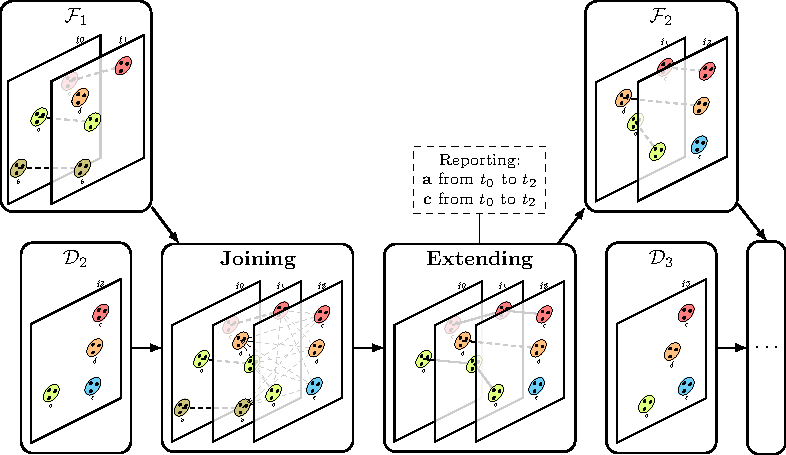
\includegraphics[width=\textwidth]{../thesis/chapterPFlocks/figures/Temporal/f_stages}
    \end{frame}

    \begin{frame}{PSI algorithm}
        \begin{minipage}{0.5\textwidth}
            \centering
            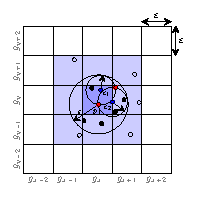
\includegraphics[width=\textwidth]{../thesis/chapterPFlocks/figures/grid_prime}
            \begin{flushright}
                {\tiny (Vieira, et al. 2009)}
            \end{flushright}
        \end{minipage}\hfill % maximize the horizontal separation
        \begin{minipage}{0.5\textwidth}
            \vspace{6mm}
            \centering
            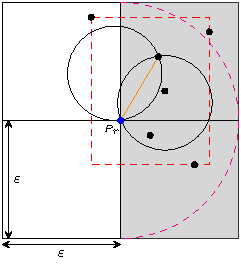
\includegraphics[width=0.78\textwidth]{../thesis/chapterPFlocks/figures/square}
            \begin{flushright}
                {\tiny (Tanaka, et al. 2016)}
            \end{flushright}
        \end{minipage}
    \end{frame}


    \begin{frame}{Challenges and contributions}
        \begin{itemize}
            \item High complexity limits scalability.
            \item Large datasets with dense clusters of moving entities per time instant significantly impact performance.
            \item Specifically,
            \begin{itemize}
                \item identifying maximal disks is hindered by the extensive number of candidates requiring pruning.
                \item when parallelizing, we must address moving flocks that traverse contiguous partitions.
            \end{itemize}
            \item We propose a parallel and scalable solution for both spatial and temporal domains.
        \end{itemize}
    \end{frame}

    \begin{frame}{On the spatial domain}
        \begin{itemize} \item Partitioning strategy... \end{itemize} \vspace{0.5cm}

         \centering
         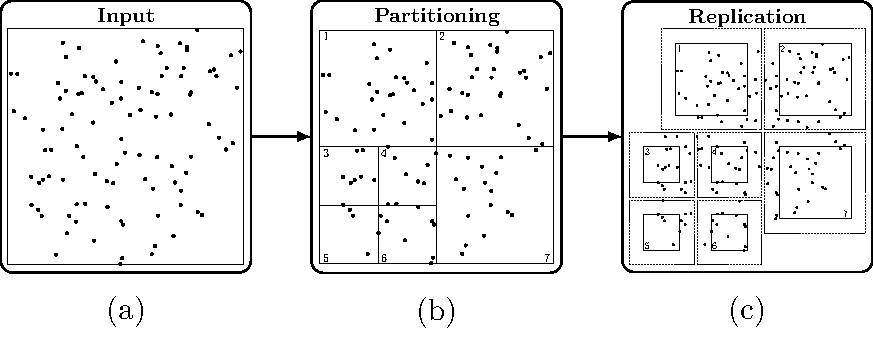
\includegraphics[trim={0 25 0 0}, clip, width=\textwidth]{../thesis/chapterPFlocks/figures/PartReplication/P123}
     \end{frame}

     \begin{frame}{On the spatial domain}
        \begin{itemize} \item Handling duplication... \end{itemize} \vspace{0.5cm}

         \centering
         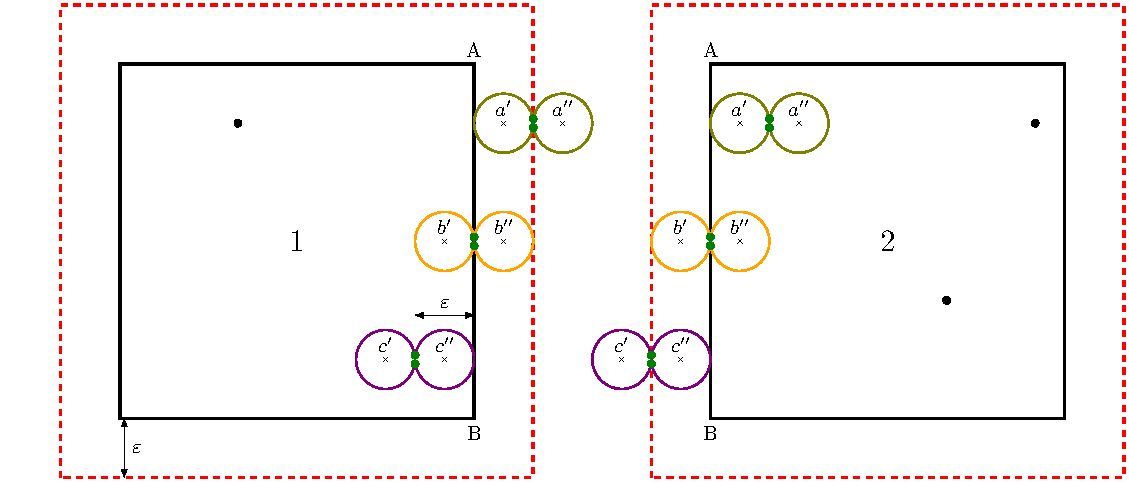
\includegraphics[width=\textwidth]{../thesis/chapterPFlocks/figures/merge}
     \end{frame}

    \begin{frame}{On the temporal domain}
            \begin{itemize} \item We introduce the \textit{maxdist} parameter to define an area were we have to track \textbf{crossing partial flocks}
(CPFs)... \end{itemize} \vspace{0.5cm}
        \centering
        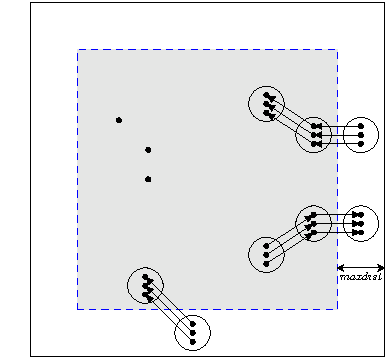
\includegraphics[height=0.6\textheight]{../thesis/chapterPFlocks/figures/maxdist}
    \end{frame}

    \begin{frame}{On the temporal domain}
        \centering
        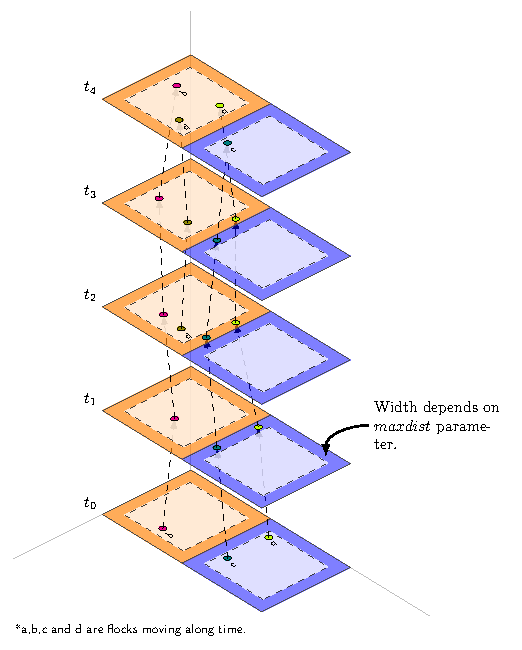
\includegraphics[height=0.9\textheight]{../thesis/chapterPFlocks/figures/plots/11_temporal_partitions/TemporalPartitioning}
    \end{frame}

    \begin{frame}{On the tempora domain}
        \begin{itemize}
            \item Discovered flocks inside the safe area are ready to be reported.
            \item CPFs require post-processing.  We propose four alternative:
            \begin{itemize}
                \item Master
                \item By-Level
                \item Least Common Ancestor (LCA)
                \item Cube-based
            \end{itemize}
        \end{itemize}
    \end{frame}

    \begin{frame}{On the temporal domain}
        \centering
        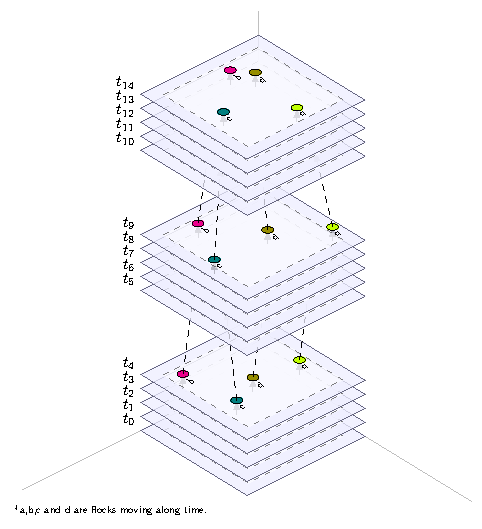
\includegraphics[height=0.9\textheight]{../thesis/chapterPFlocks/figures/plots/11_temporal_partitions/Cube-based}
    \end{frame}

    \begin{frame}{Datasets}
            \centering
            \begin{tabular}{cccc}
                \hline
                        & Number of    & Total number & Maximum        \\
                Dataset & Trajectories & of points    & Duration (min) \\
                \hline
                Berlin10K &  10000 & 97526 & 10\\
                LA25K &  25000 & 1495637 & 30\\
                LA50K &  50000 & 2993517 & 60\\
                \hline
            \end{tabular}
     \end{frame}

     \begin{frame}{Datasets}
        \begin{itemize} \item Synthetic datasets [LA50K] \end{itemize} \vspace{0.25cm}

         \centering
         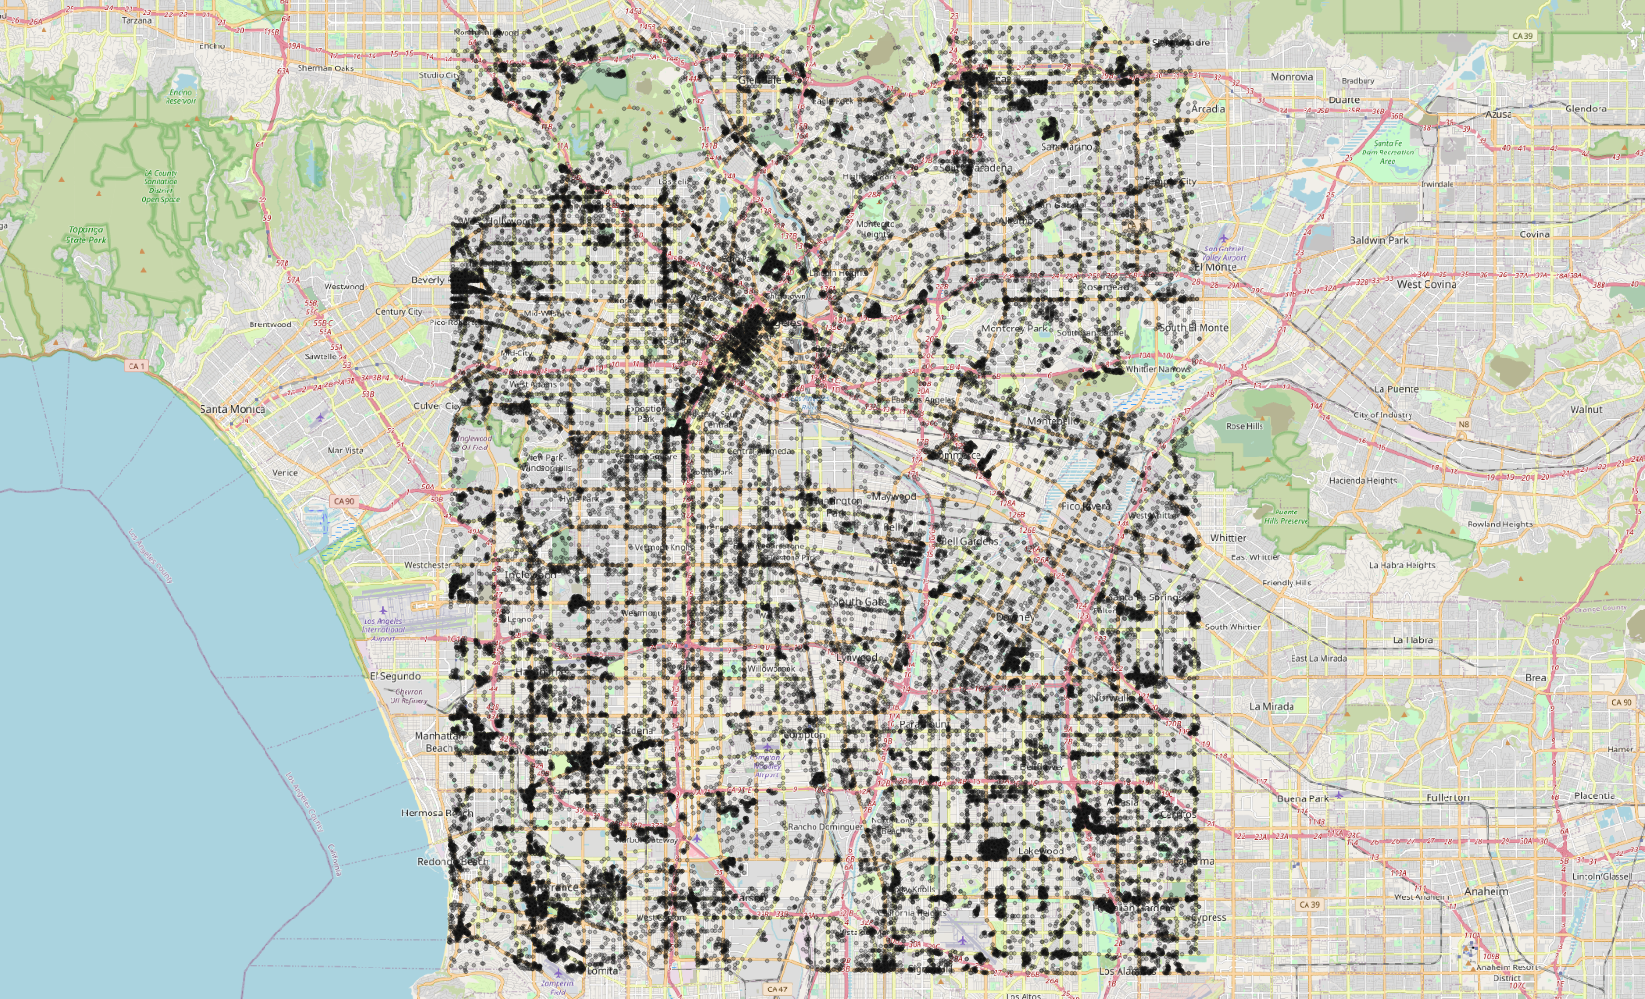
\includegraphics[width=\textwidth]{figures/LA_T320_N50K.png}
     \end{frame}

    \begin{frame}{Experiments}
        \begin{itemize} \item Optimizing the number of partitions for Phase 1. \end{itemize} \vspace{0.5cm}

        \begin{figure}
            \centering
            \begin{subfigure}[t]{0.32\textwidth}
                \raisebox{-\height}{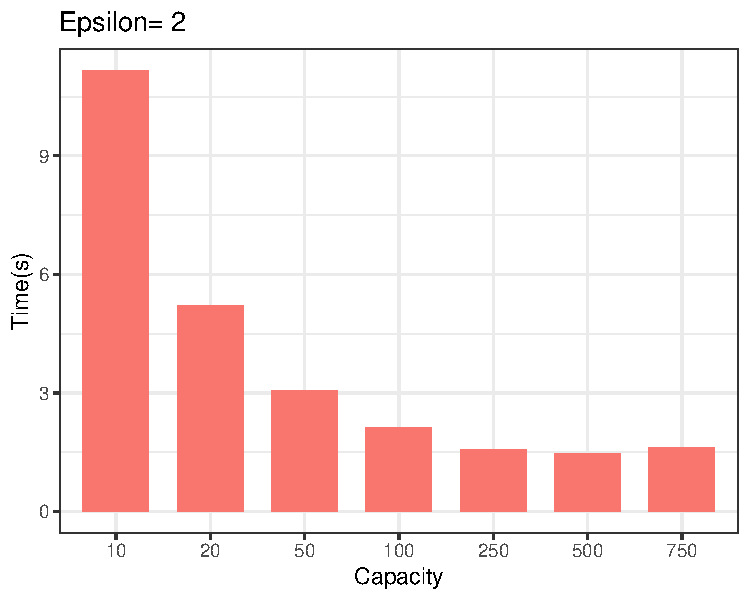
\includegraphics[width=\textwidth]
                {../thesis/chapterPFlocks/figures/plots/01_optimal_performance/pflockE2_by_capacity}}
            \end{subfigure}
            \hfill
            \begin{subfigure}[t]{0.32\textwidth}
                \raisebox{-\height}{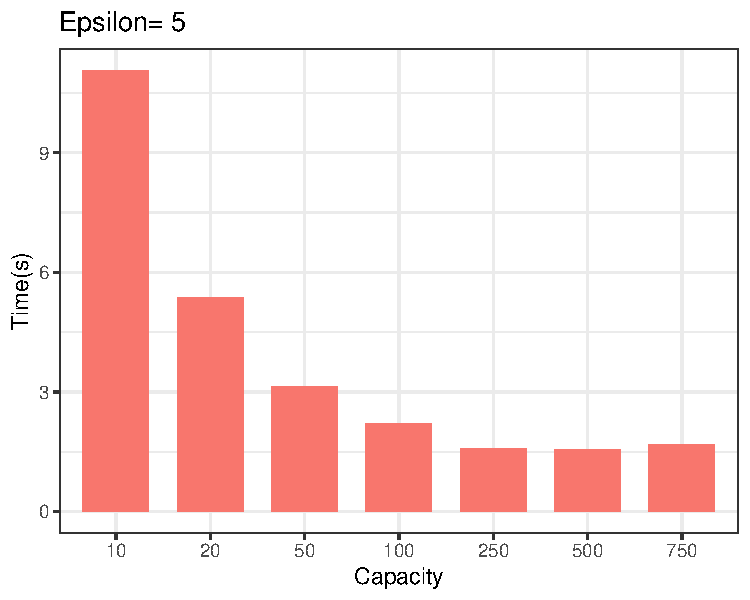
\includegraphics[width=\textwidth]
                {../thesis/chapterPFlocks/figures/plots/01_optimal_performance/pflockE5_by_capacity}}
            \end{subfigure}
            \hfill
            \begin{subfigure}[t]{0.32\textwidth}
                \raisebox{-\height}{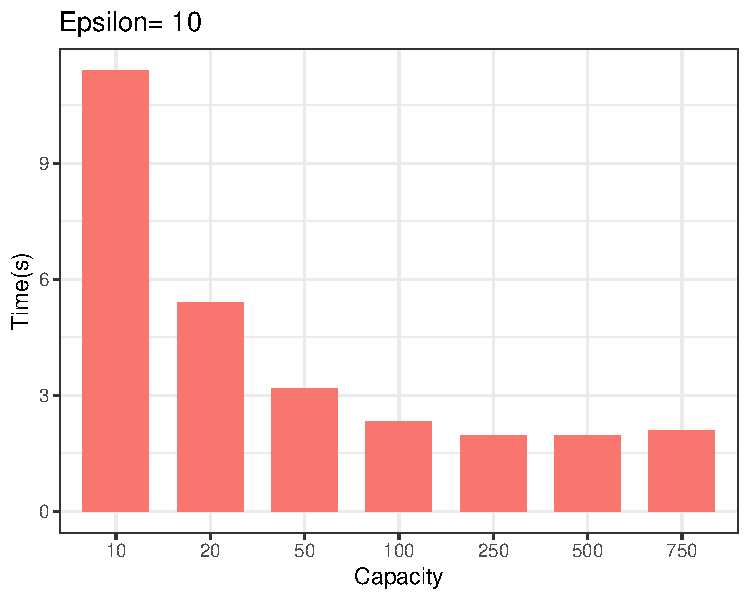
\includegraphics[width=\textwidth]
                {../thesis/chapterPFlocks/figures/plots/01_optimal_performance/pflockE10_by_capacity}}
            \end{subfigure}
            %%%%%%%%%%%%%%%%%%%%%%%%%%%%%%%%%%%%second row
            \begin{subfigure}[t]{0.32\textwidth}
                \raisebox{-\height}{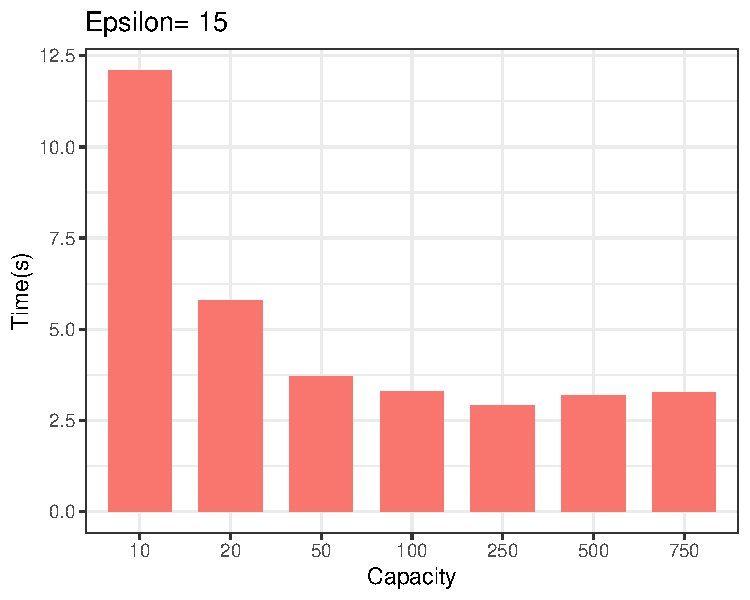
\includegraphics[width=\textwidth]
                {../thesis/chapterPFlocks/figures/plots/01_optimal_performance/pflockE15_by_capacity}}
            \end{subfigure}
            %\hfill
            \begin{subfigure}[t]{0.32\textwidth}
                \raisebox{-\height}{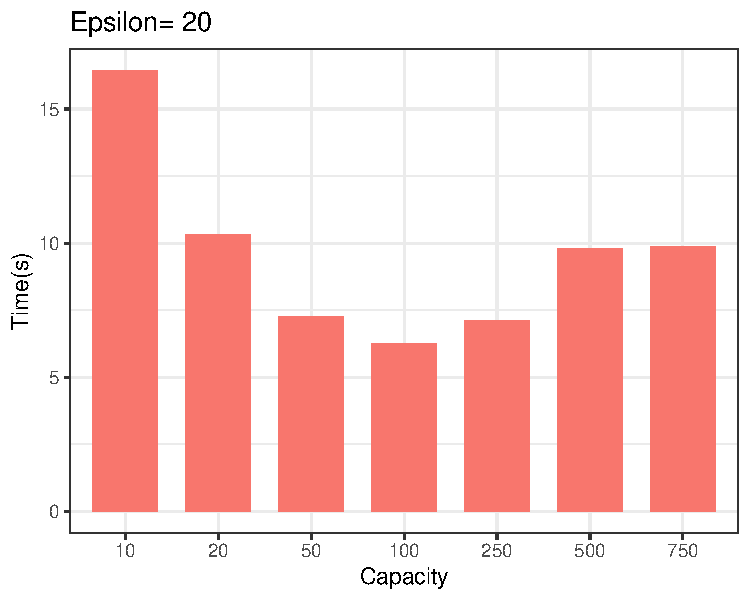
\includegraphics[width=\textwidth]
                {../thesis/chapterPFlocks/figures/plots/01_optimal_performance/pflockE20_by_capacity}}
            \end{subfigure}
        \end{figure}
    \end{frame}

    \begin{frame}{Experiments}
        \begin{itemize} \item Analyzing most costly partitions.
            \begin{itemize}
                \item Top 10 most costly partitions.
            \end{itemize}
        \end{itemize} \vspace{0.25cm}

        \centering
        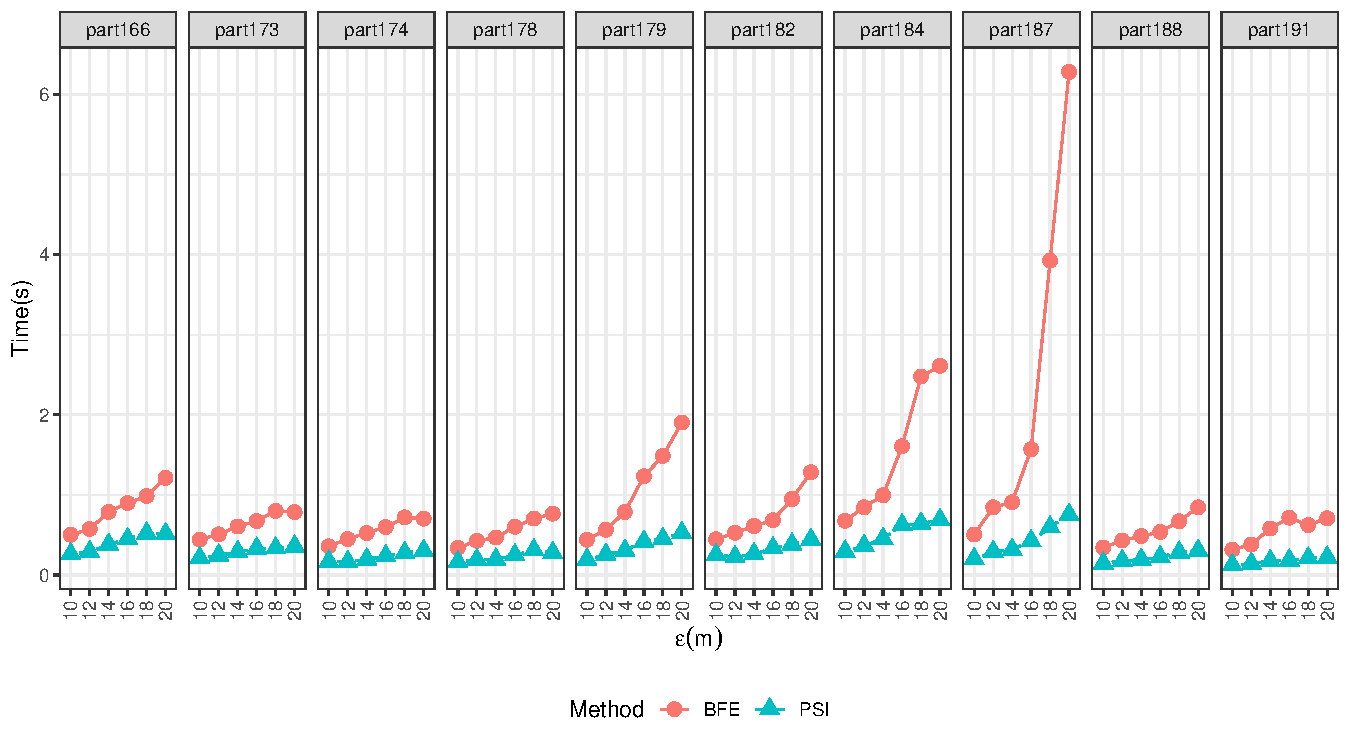
\includegraphics[width=\textwidth]
                {../thesis/chapterPFlocks/figures/plots/03_top_time_partitions/top_time_partitions}

    \end{frame}

    \begin{frame}{Experiments}
        \begin{itemize} \item Analyzing most costly partitions.
            \begin{itemize}
                \item By Pairs density..
            \end{itemize}
        \end{itemize} \vspace{0.25cm}

        \centering
        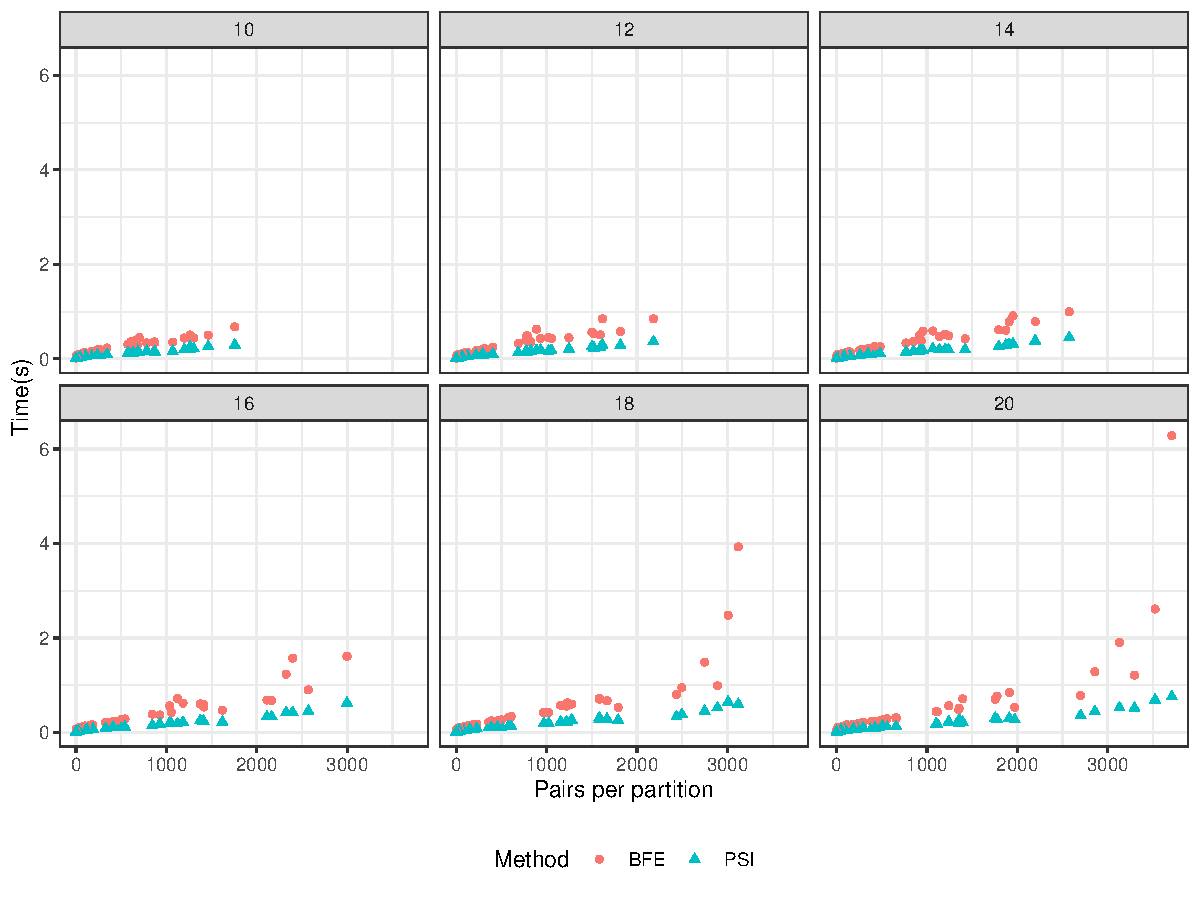
\includegraphics[width=0.8\textwidth]
                {../thesis/chapterPFlocks/figures/plots/04_pairs_performance/pairs_performance}
    \end{frame}

    \begin{frame}{Experiments}
        \begin{itemize} \item Analyzing most costly partitions.
            \begin{itemize}
                \item By Stages in the most costly partition [(a) BFE (b) PSI].
            \end{itemize}
        \end{itemize} \vspace{0.25cm}

        \centering
        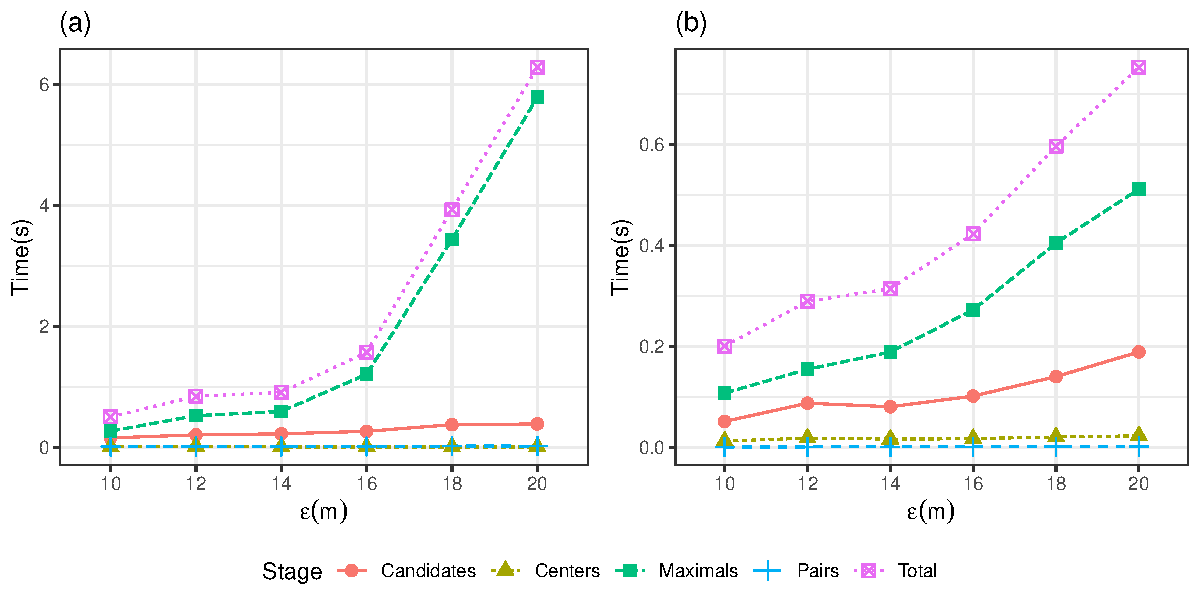
\includegraphics[width=\textwidth]
                {../thesis/chapterPFlocks/figures/plots/09_dense_stages/dense}
    \end{frame}

    \begin{frame}{Can we reduce pruning time?}
        \begin{itemize}
            \item \textbf{Maximal clique (MC)}: Given an undirected graph, a MC is a subset of vertices, each directly connected to every other in the subset,
that cannot be expanded by adding additional vertices.
            \item \textbf{Minimum Bounding Circle (MBC)}: Given a set of points in Euclidean space, the MBC is the smallest circle that can enclose all the
points.
        \end{itemize}
    \end{frame}

    \begin{frame}{Can we reduce pruning time?}
        \centering
        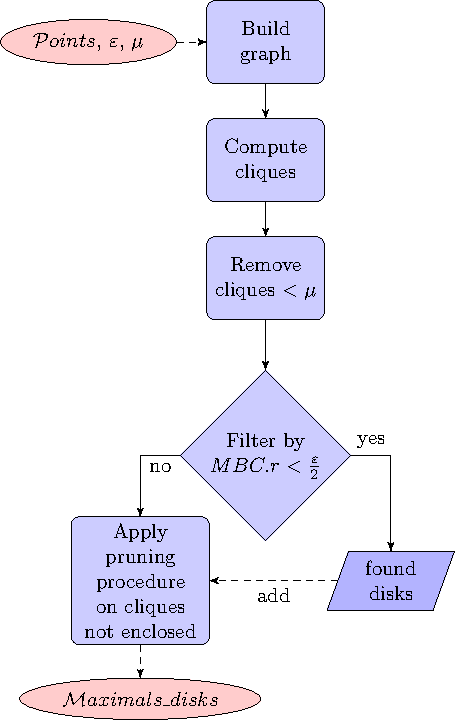
\includegraphics[height=0.85\textheight]
                {../thesis/chapterPFlocks/figures/plots/10_cmbc_variants/CMBC_flowchart2}
    \end{frame}

    \begin{frame}{Can we reduce pruning time?}
        \begin{itemize}
            \item Phase 1 variants performance [(a) vs BFE (b) vs PSI].
        \end{itemize} \vspace{0.25cm}

        \centering
        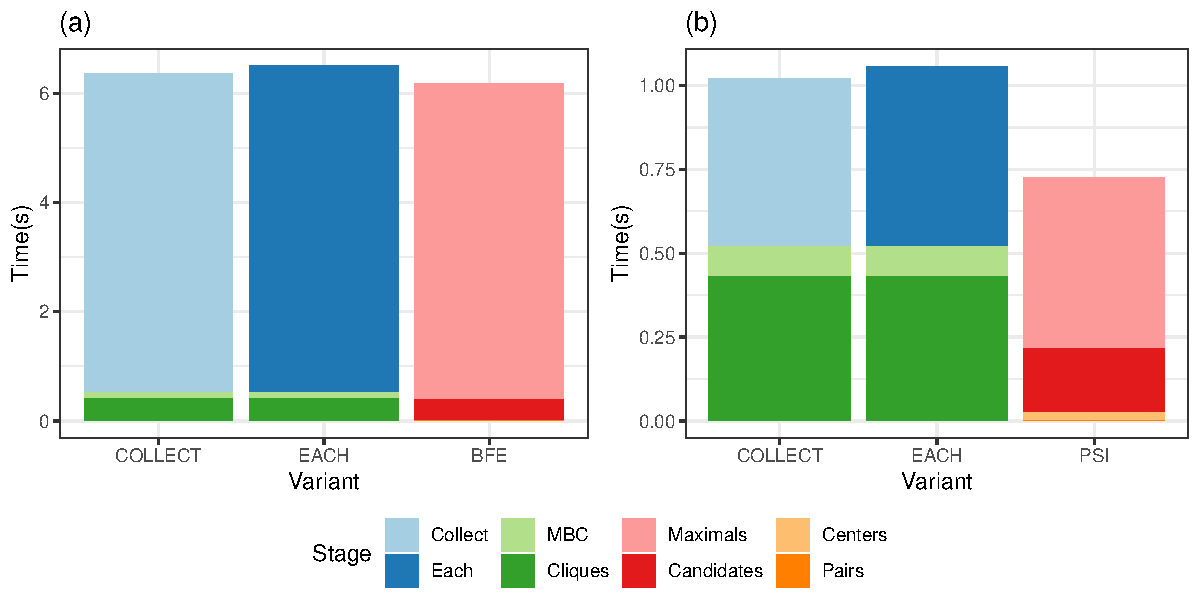
\includegraphics[width=\textwidth]
                {../thesis/chapterPFlocks/figures/plots/10_cmbc_variants/cmbc}
    \end{frame}

    \begin{frame}{Experiments}
        \begin{itemize}
            \item Relative performance of Phase 1 using synthetic datasets.
        \end{itemize} \vspace{0.25cm}

        \centering
        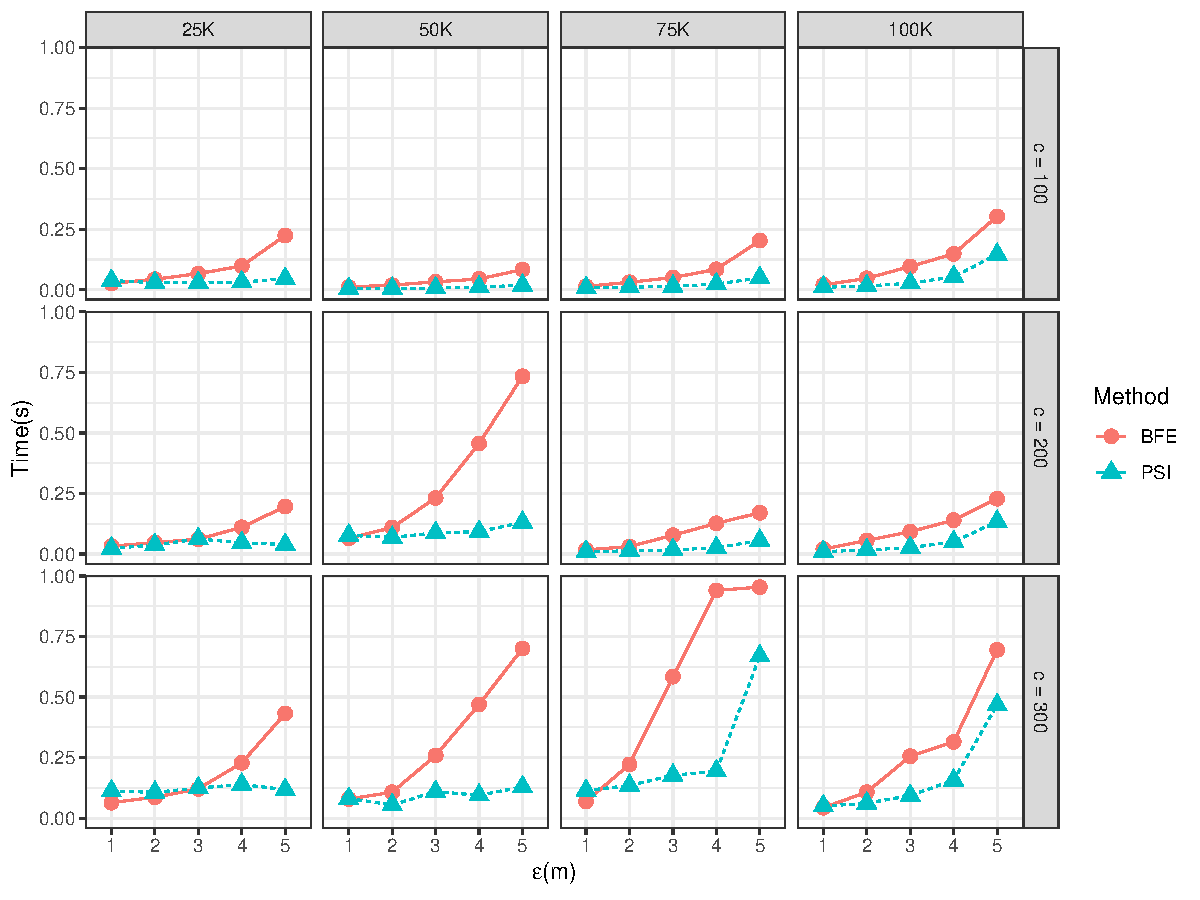
\includegraphics[width=0.8\textwidth]
                {../thesis/chapterPFlocks/figures/plots/05_uniform_performance/uniform_performance}
    \end{frame}

    \begin{frame}{Experiments}
        \begin{itemize}
            \item Finding best \textit{step} value for By-Level alternative.
        \end{itemize} \vspace{0.25cm}

        \centering
        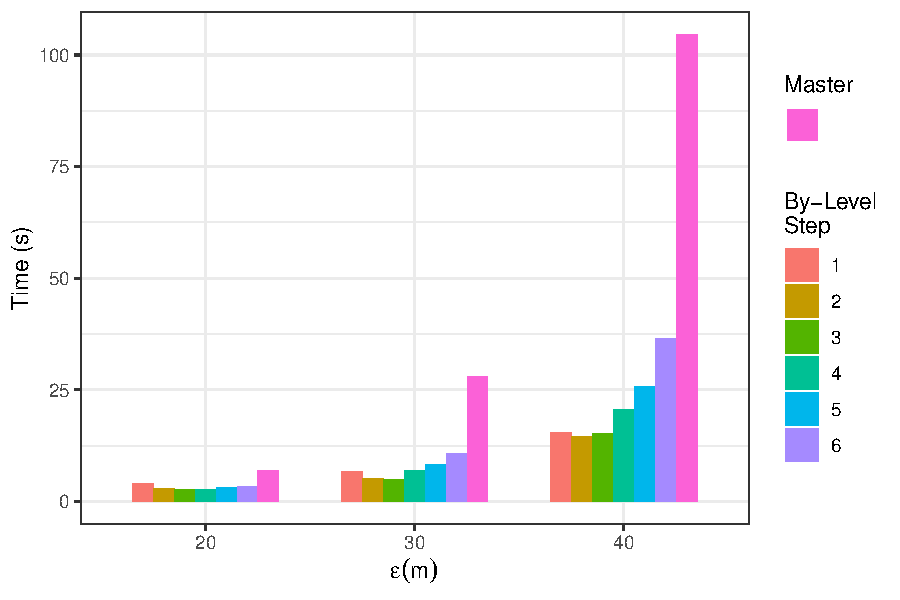
\includegraphics[width=0.9\textwidth]
                {../thesis/chapterPFlocks/figures/plots/06_step_performance/step_performance}
    \end{frame}

    \begin{frame}{Experiments}
        \begin{itemize}
            \item Finding best \textit{interval} value for Cube-based alternative.
        \end{itemize} \vspace{0.25cm}

        \centering
        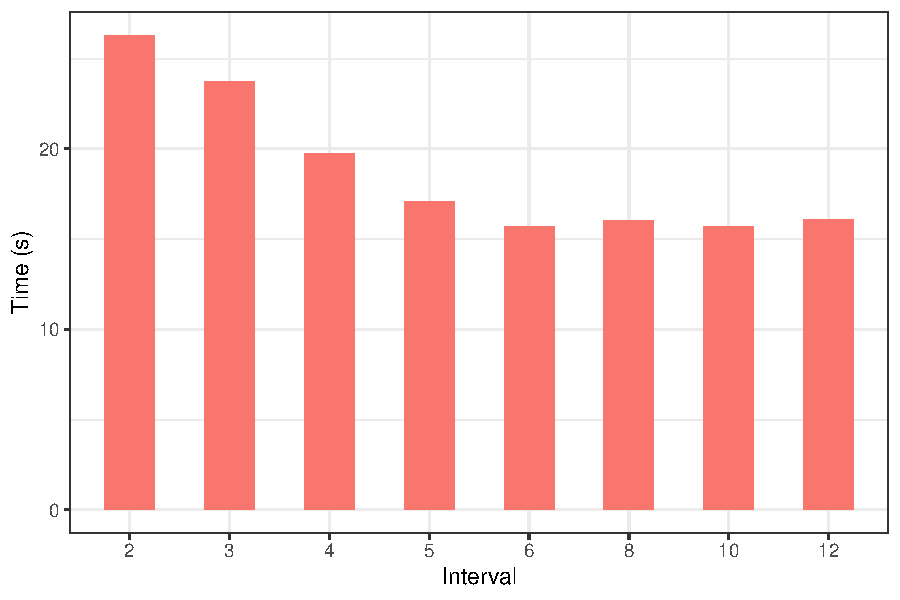
\includegraphics[width=0.9\textwidth]
                {../thesis/chapterPFlocks/figures/plots/07_interval_performance/interval-performance}
    \end{frame}

    \begin{frame}{Experiments}
        \begin{itemize}
            \item Scalable alternatives vs standard PSI.
        \end{itemize} \vspace{0.25cm}

        \centering
        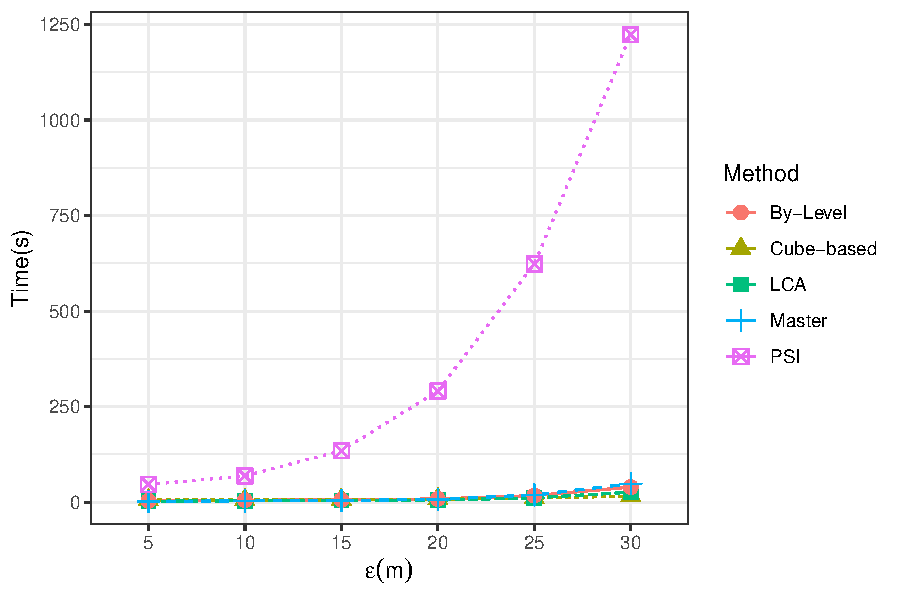
\includegraphics[width=0.9\textwidth]
                {../thesis/chapterPFlocks/figures/plots/08_sequential_parallel/la25k_e_bfe_psi}
    \end{frame}

    \begin{frame}{Experiments}
        \begin{itemize}
            \item Scalable alternatives in LA25K dataset.
        \end{itemize} \vspace{0.25cm}

        \centering
        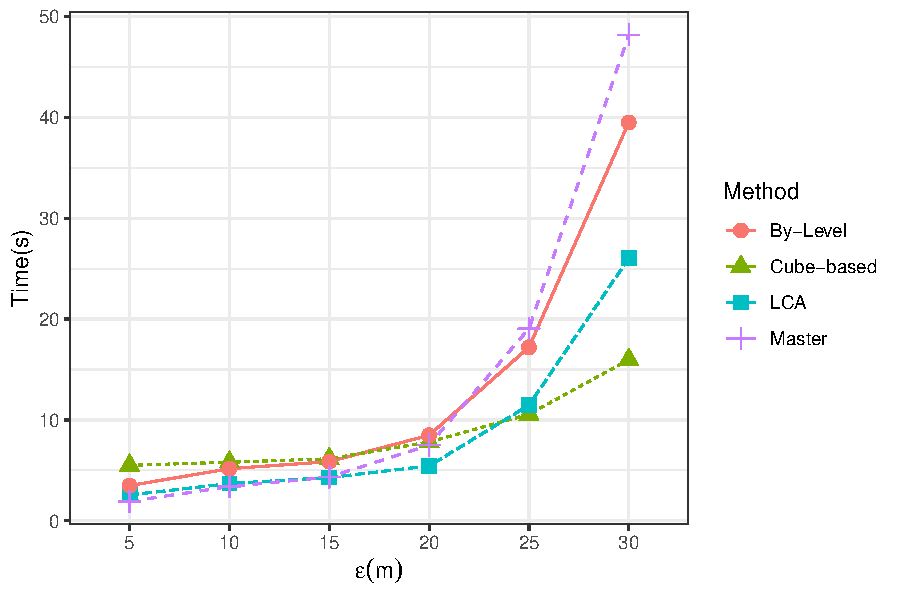
\includegraphics[width=0.9\textwidth]
                {../thesis/chapterPFlocks/figures/plots/08_sequential_parallel/la25k_e}
    \end{frame}

    \begin{frame}{Experiments}
        \begin{itemize}
            \item Scalable alternatives in LA50K dataset.
        \end{itemize} \vspace{0.25cm}

        \centering
        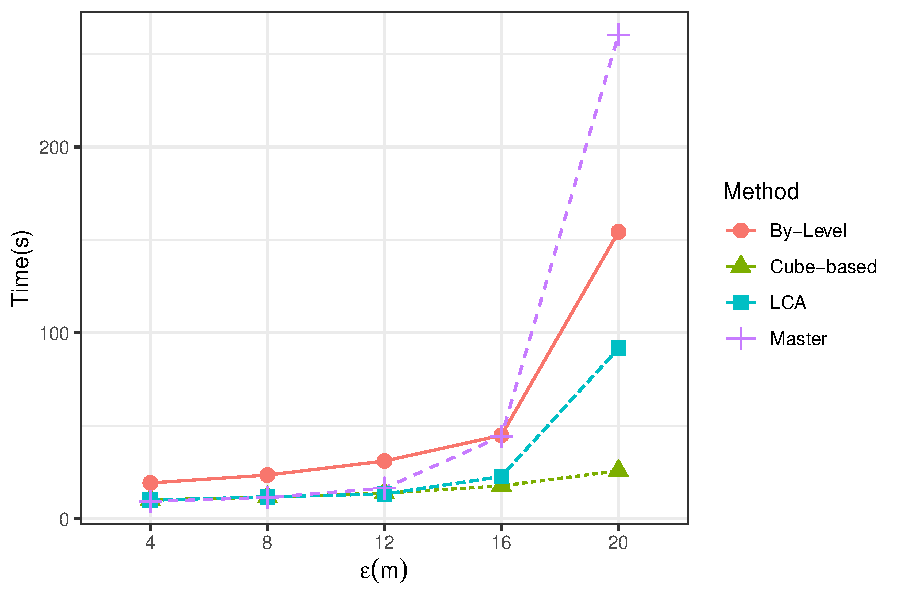
\includegraphics[width=0.9\textwidth]
                {../thesis/chapterPFlocks/figures/plots/08_sequential_parallel/la50k_e}
    \end{frame}
